\section{Sơ đồ tổng thể của pipeline}
\label{sec:4_1}
Sau khi khóa cách chia tập, dữ liệu đầu vào được tách thành sáu biến số và tám biến phân loại. Hai nhánh xử lý được ghép lại, có thể đi qua PCA, rồi chuyển thành ma trận \texttt{float32}. Nhãn \texttt{income} và các cột metadata không tham gia fit đặc trưng.

\begin{figure}[htbp]
\centering
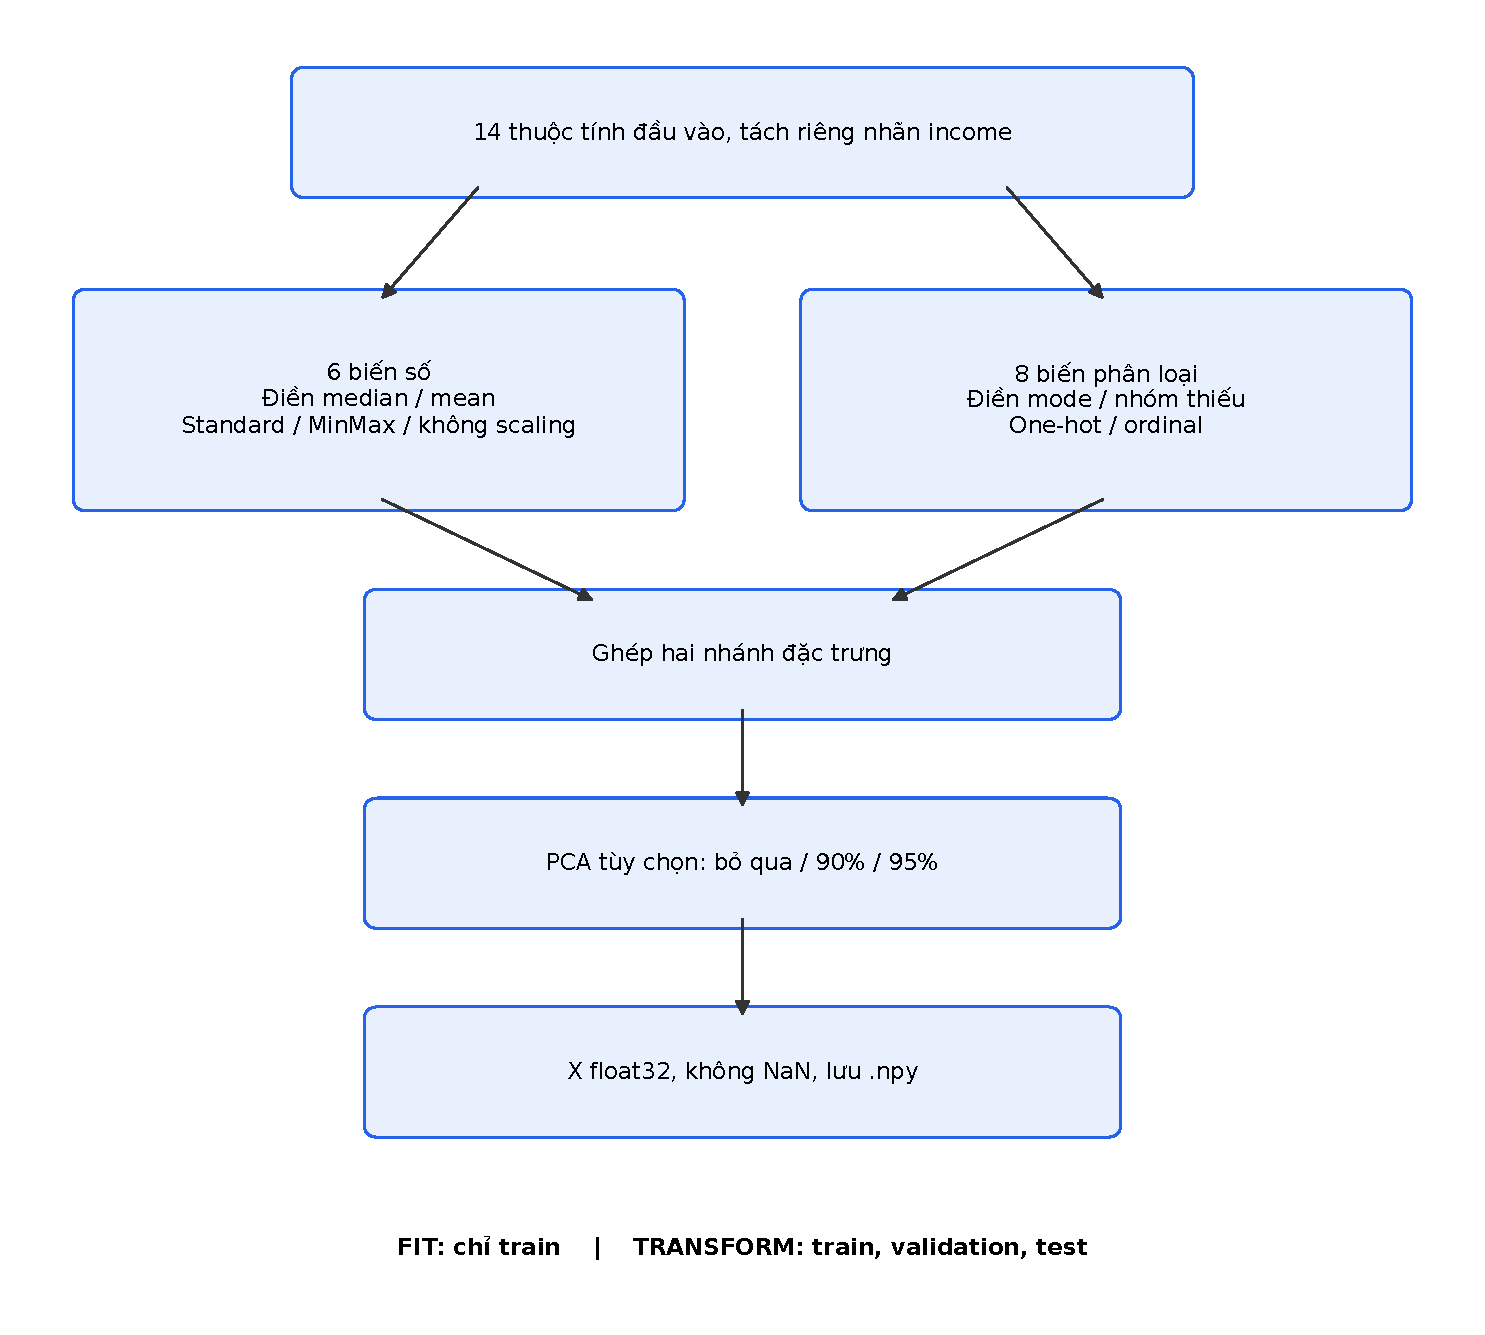
\includegraphics[width=.88\textwidth,height=.76\textheight,keepaspectratio]{Images/chapter_4/4_1/preprocessing_pipeline.pdf}
\caption{Cấu trúc pipeline tiền xử lý; tất cả bước học tham số chỉ fit trên train}
\label{fig:preprocessing-pipeline}
\end{figure}

Phần chuẩn bị đặc trưng có thể được xuất độc lập thành các ma trận NumPy. Khi thực nghiệm mô hình, bộ tiền xử lý chưa fit được ghép với bộ phân loại trong một pipeline hoàn chỉnh để fit đúng phạm vi dữ liệu của từng fold. Sau lựa chọn bằng CV, pipeline được fit trên toàn bộ train và giữ cố định để đánh giá cuối.
